\section {Method}

\subsection {Mach-Zenhder setup}
This setup for the Mach-Zendher interferometer with phase shifting consists of
a laser (Melles Griot, 05-LHP-111), which is chosen for its long coherens length. 
If we had used white light the components would have to been placed with micrometer 
precision. Using a laser gives a coherens length of about a meter. Though it will 
create noise in the measurements which needs to be weighed in.
The laser beam goes through a beam expander, which due to the nature of lasers having 
a gaussian distribution of intensity, and us wanting a uniform distribution, 
we expand the laser and use only the middle of the beam.
A beam splitter splits the laser beam in two, sending one to a piezo controlled
mirror. 
The piezo is controlled by a computer sending signals to a Nidaq 
(National Instruments, NI USB-6211) which is connected to a high voltage DC OP amp
(burleigh, PZ-70) converting a voltage in a range of -10 V to 10 V 
into 500 V to 1000 V. This gives high precision control of the movement of the 
mirror down to about the order of 10 nm, thus making it possible to move the 
phase of the light wave with great accuracy. From the piezo mirror it is sent 
through a sample cell which contains what we are measuring.
Then it is sent to a beam collector and the interference pattern is picked up by
a CCD camera (Imaging Source, DMK 21BUC03) which is connected to a computer who stores the data.
The second beam travels without hinderance to the collector.

\subsection {Unwrapping}
To analyze the data coming from the camera we used a method called unwrapping.
As we only get an intensity from the camera we have to translate this into something
we can use to analyze the motion of the phase picture. Most of this section
is collected from Optical Measurement of Surface Topography.\cite{omst} 
The interference signal can be expressed as:
\begin {equation}
I(\phi) = I_{DC} + I_{AC}\cos[\theta + \phi]
\end {equation}
where $I_{DC}$ and $I_{AC}$ are fixed coefficients and $\theta$ is the phase and
$\phi$ is the phase shift in terms of the reference mirror displacement.
This equation can then be expanded to
\begin {equation}
I(\phi) = I_{DC} + I_{AC}[\cos(\theta)\cos(\phi) - \sin(\theta)\sin(\phi)]
\end {equation}
Fitting the sine and cosine waves to the interference signal gives the $\sin(\theta)$
and $\cos(\theta)$ terms.
To get the wanted $\theta$ out of this equation it is possible to integrate over
a full cycle of phase $\phi$
\begin {align}
N &= -\int_{-\pi}^{\pi}I(\phi)\sin(\phi)d\phi\\
D &= \int_{-\pi}^{\pi}I(\phi)\cos(\phi)d\phi
\end {align}
Then the phase $\theta$ can be extracted with
\begin {equation}
\tan(\theta) = N/D
\end {equation}
The signal $I(\phi)$ is what we are measuring in the camera and thus by shifting
$\phi$ with evenly placed discrete values $\Delta\phi = \pi/2$ the equation above
becomes
\begin {align}
N &= I_0 +I_1 - I_2 + I_3\\
D &= -I_0 + I_1 + I_2 - I_3
\end {align}
and we get 
\begin {equation}
\tan(\theta) = \frac{I_0 - I_2}{-I_0 + 2I_1 - I_2}
\end {equation}
This can be done for more intensity samples as well, and thus for 7, as we used,
we get
\begin {equation}
\tan(\theta) = \frac{2I_1 - 2I_3}{-I_0 + 2I_2 - I_4}
\end {equation}
By taking the $\arctan$ of this equation we are left with the shifted phase.
But due to the nature of $\tan$, the picture will only have a range of $2\pi$
and therefore have false drops. 
\begin {figure}[ht!]
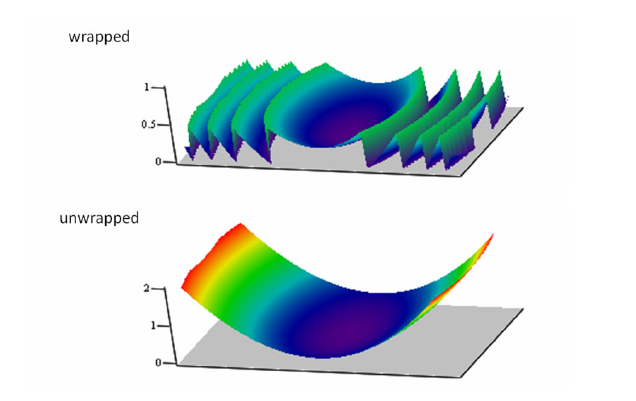
\includegraphics [width=10cm]{bilder/unwrap.png}
\caption {\cite{omst}An illustrative graph of a wrapped and unwrapped phase picture respectivly 
with unit length on the x and y axis, z in radians.}
\end {figure}
To correct these drops we used a 2 dimensional unwrapping algorithm in Matlab called
Constantini phase unwrapping which is based on an article written by M. Constantini 
\cite{const}. This unwrapping of the phase gives a picture of how the phase $\theta$ is moving
as $\phi$ is changed. 

\subsection {Diffusion of table salt in water}

The reason for this experiment was to test the equipment to see if every component
could work together and also get an approximation of how well the accuracy is.
We expected to see an inclination rising as the salt diffused into the water since
the optical path length rises when the water and salt gets mixed.
To be able to control the phase shift with the piezo we did a callibration to find
which voltage represented one wavelength. By using the background it was measured to
be a factor of 1.12 which we multiplied to the signal out to the Nidaq. Then we placed a rectangle 
sided vial with clear plastic in the middle in front of the beam.

\begin {figure}[ht!]
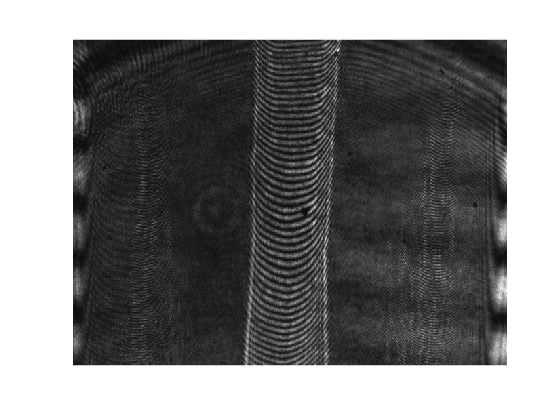
\includegraphics [width=10cm]{bilder/sample.png}
\caption {A vial with nothing in it. The black and white stripes are the inteference %
          of the beam because of the difference in optical path length compared to the %
          unhindered beam. At the far sides there is a background inteference pattern %
          which arise from the camera not being completely aligned.}
\end {figure}

The vial were filled with 2.16 g of water and a piece of 3 mg of salt was added to it,
and a Matlab code took a picture about every 2 minutes depending on how long the 
unwrapping algorithm took. This went on overnight and we got around 300 measurements.
\begin {figure}[ht!]
\begin {subfigure}[h]{0.35\textwidth}
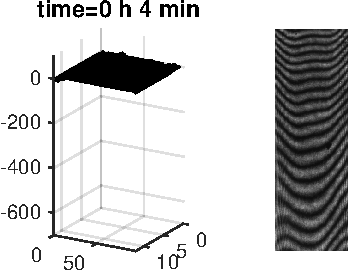
\includegraphics [width=5cm]{bilder/diff2.pdf}
\caption {The first image taken after starting the experiment. To th right is the
unwrapped phase subtracted from the background giving it a zero value. On the z-axis
the phase is plotted in radians and the x-y plane is in pixels. To the right
is the image from the camera.}
\end {subfigure}
\hfill
\begin {subfigure}[h]{0.35\textwidth}
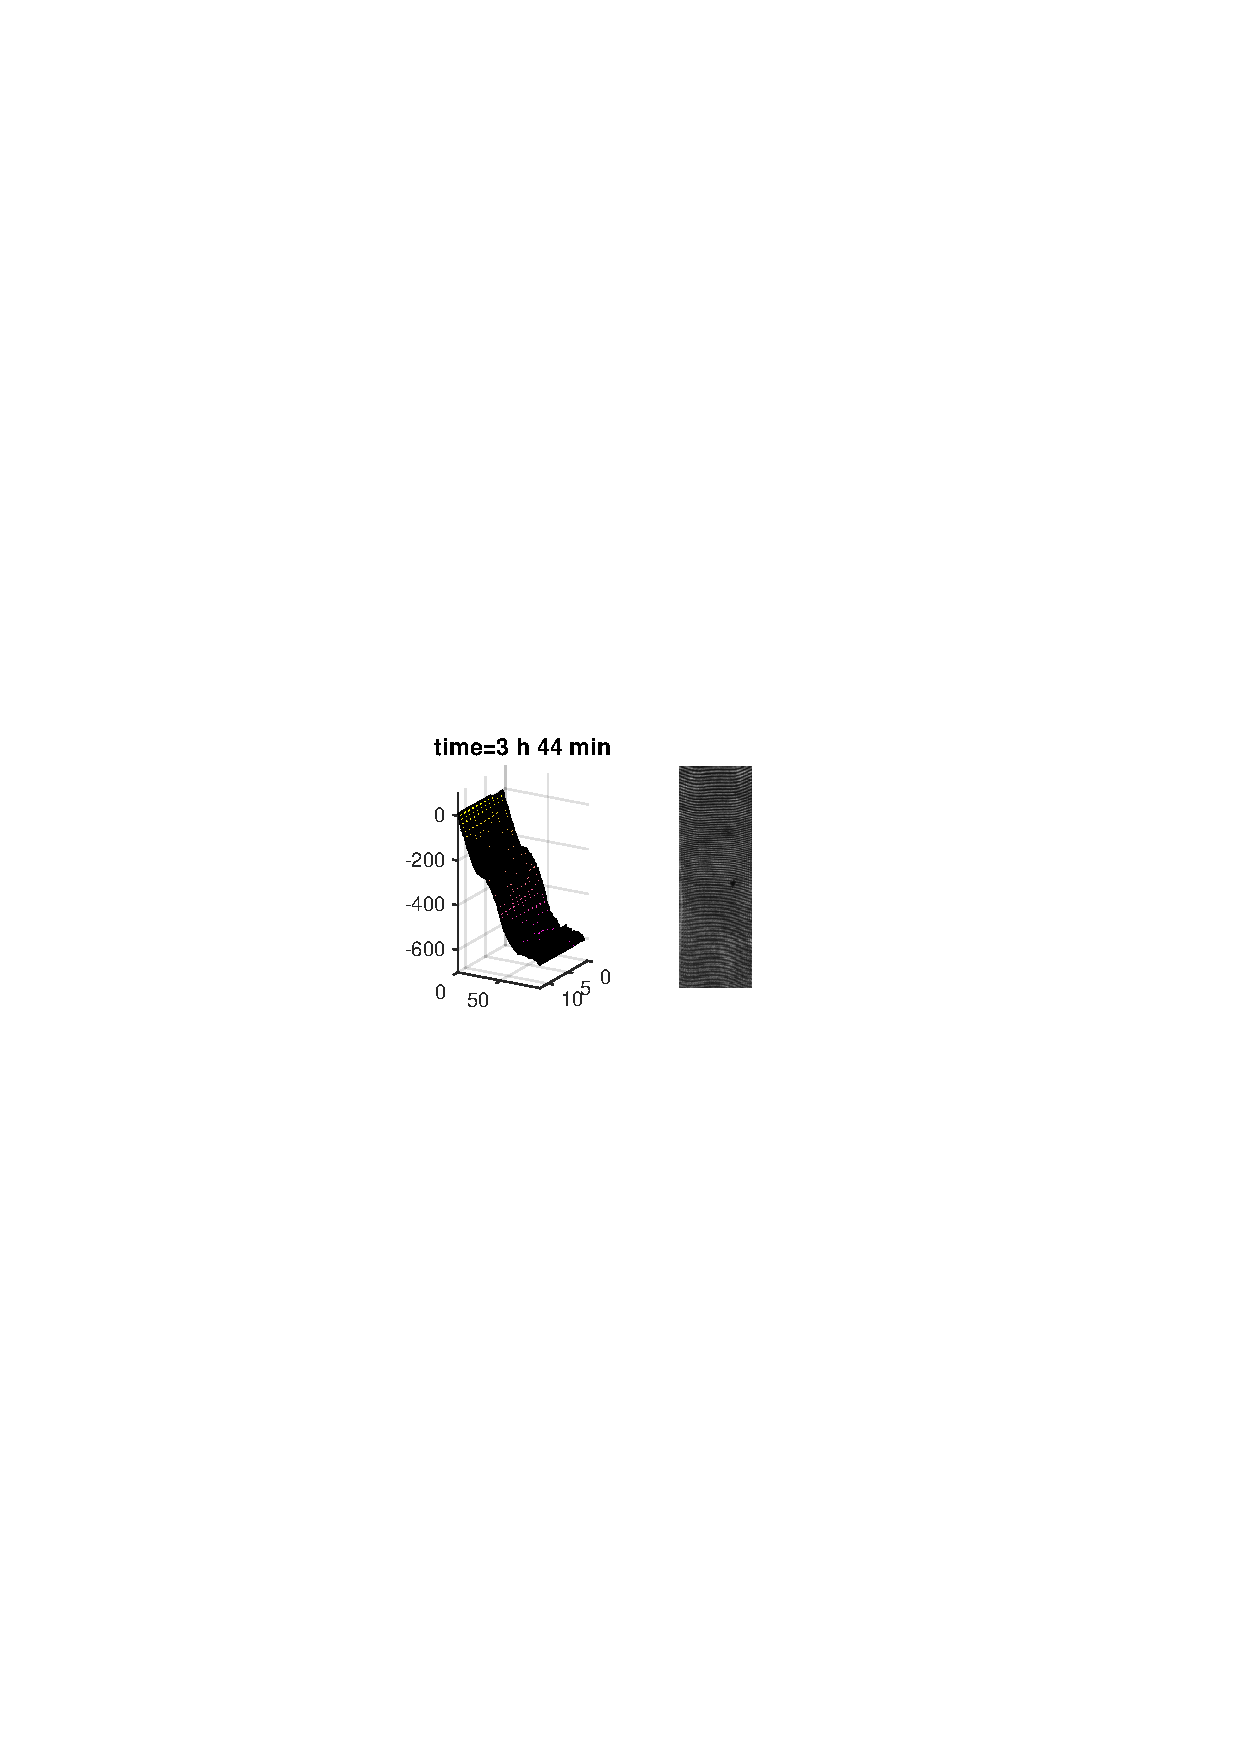
\includegraphics [width=5cm]{bilder/diff102.pdf}
\caption {After almost 4 hours the salt has diffused into the solution and the phase
has become a lot steeper. As seen on the camera the number of fringes has increased
significantly. There are also some optical effects due to too much salt as one can
see in both the phase and the camera.}
\end {subfigure}

\begin {subfigure}[h]{0.35\textwidth}
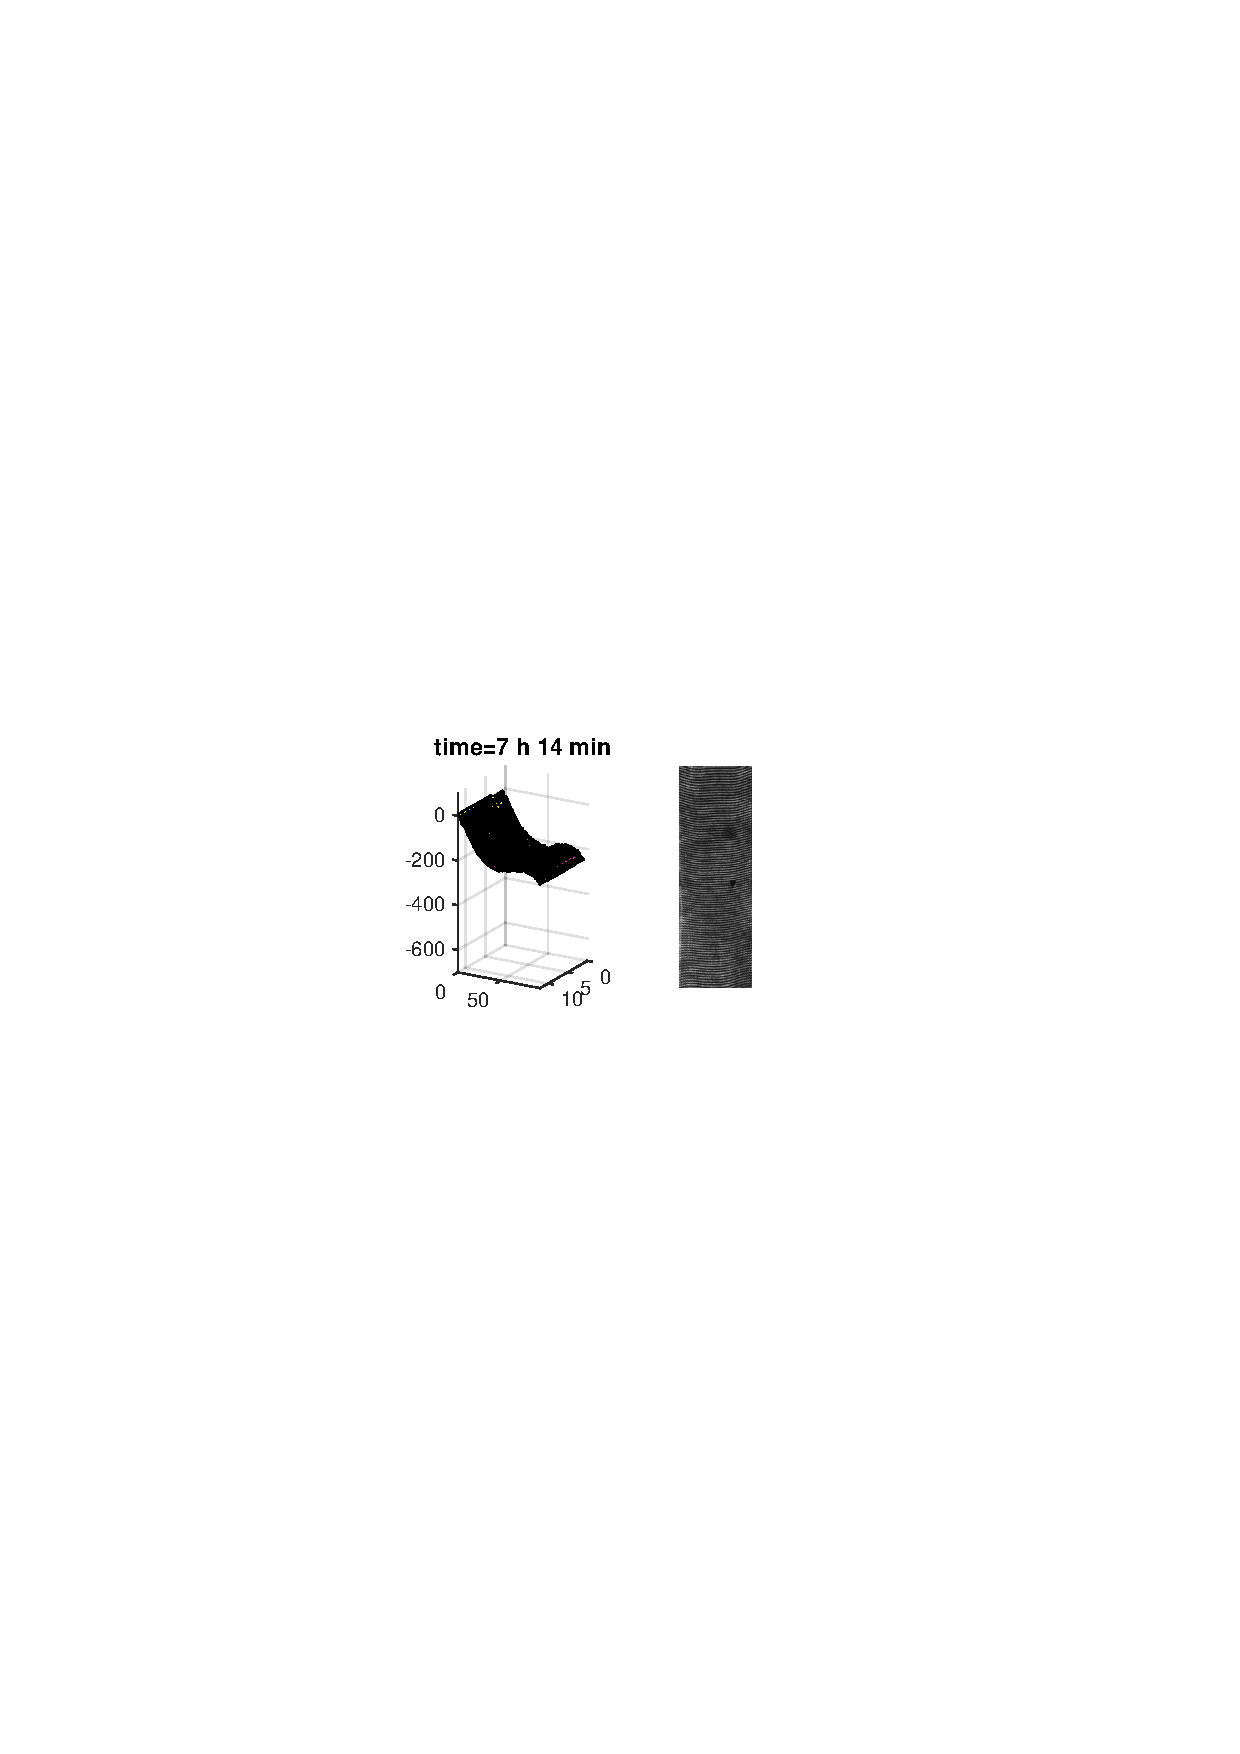
\includegraphics [width=5cm]{bilder/diff202.pdf}
\caption {7 hours in the phase is showing some warped behaviour due to the salt amount}
\end {subfigure}
\hfill
\begin {subfigure}[h]{0.35\textwidth}
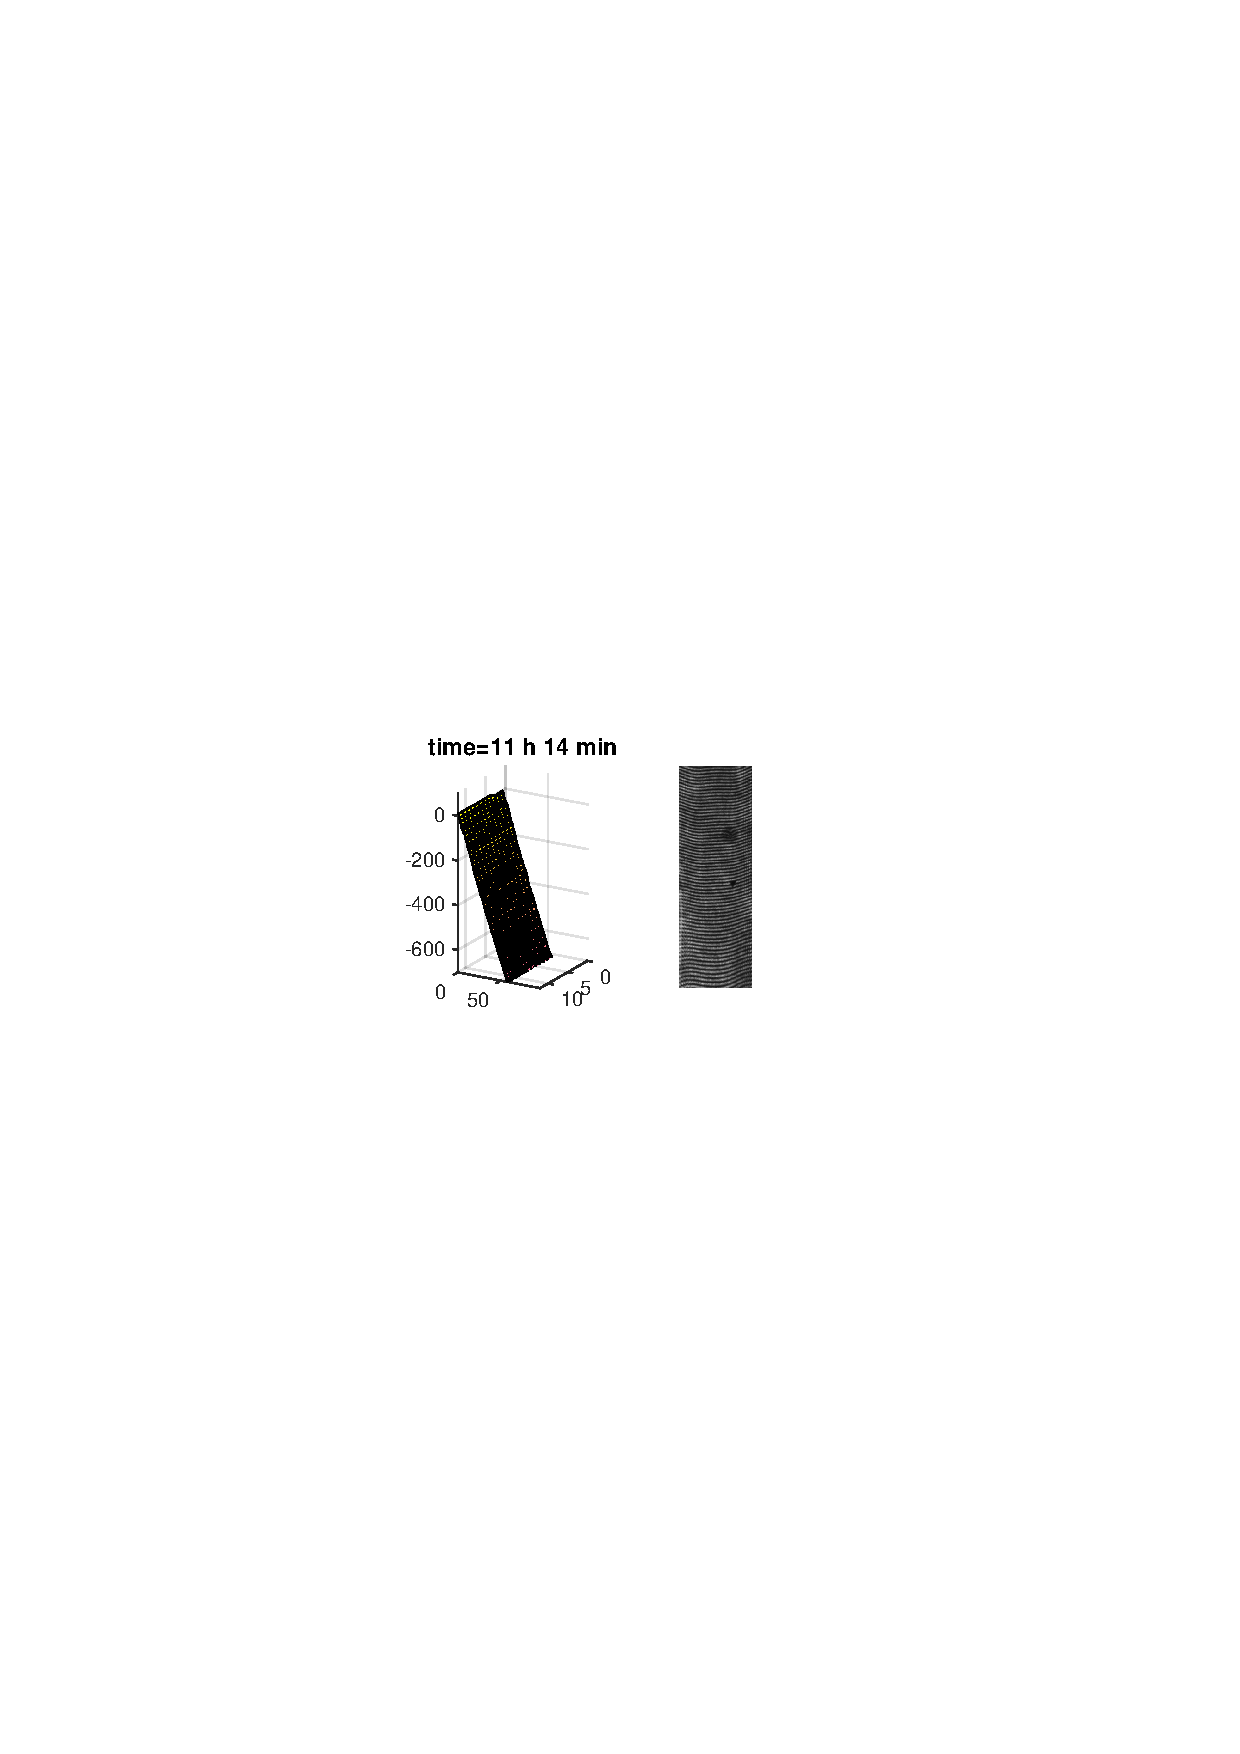
\includegraphics [width=5cm]{bilder/diff302.pdf}
\caption {11 hours into the experiment the solution has quiet down and shows a
steep inclination compared to the background which is expected since the optical
path length is higher in salt water then in pure water}
\end {subfigure}
\end {figure}
%Sett inn bildeserie

\subsection {Calcit erosion by water}

The goal of this experiment was to get an estimate of how accurate this setup can be.
We want to see an erosion beginning in the start of the canal and have an exponential
difference in optical path length along the canal as the erosion takes place.
It is expected to be a steep inclination in the beginning of the unwrapping picture
and as the experiment goes on, the inclination should spread to the entire picture.

\begin {figure}[ht!]
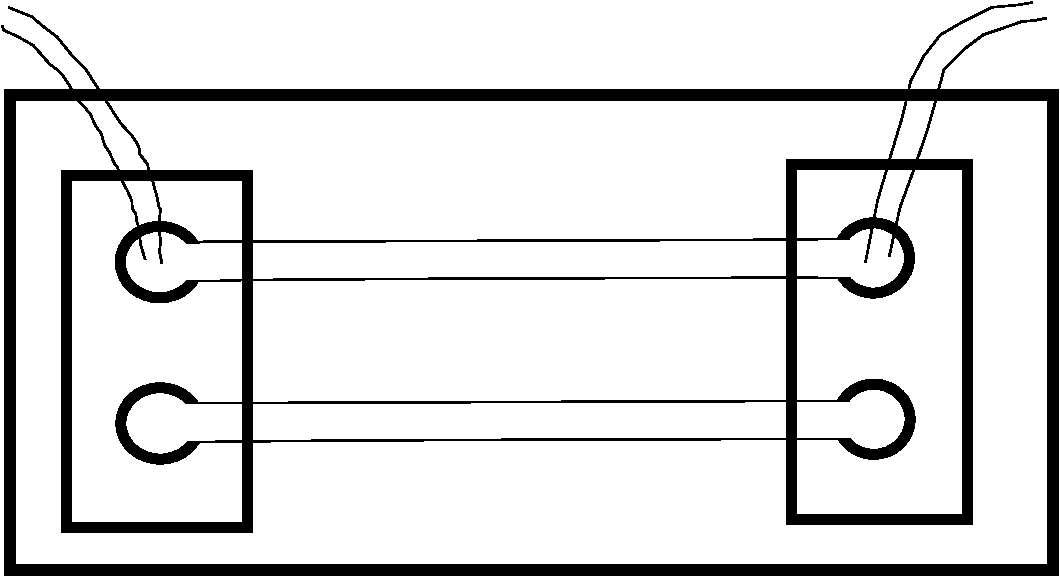
\includegraphics [width=10cm]{bilder/calcitsample.pdf}
\caption {%
It was made of a calcit sample by taking a plexi glass surface, bore four holes
in it and two other plexi cubes. Then using a special sticker with glue on it to
fasten the calcit to the plexi surface and creating two canals, with a wdith of about
300 $\mu$m, between the glass and the calcit. Two plastic tubes are threaded down 
on each side of a canal through the plexi cubes so it can deliver a water stream 
through the canals.}
\end {figure}

The water delivery system was a syringe put on an automated pump 
(kdScientific, LEGATO 180). 
We set the pump to 10 nl/s and started the same Matlab program as with the diffusion
experiment only with about 5 minute spaces between the measurements and the experiment
went on for about 24 hours. The second experiment was with the same paramaters but with 
added salt peter acid to the water to get a larger erosion rate. The unwrapping of
the phase were done in the area from 5 pixels above to 5 pixels below the canal, 
and the canal before the erosion was about 2 pixels wide.

%\begin {figure}[ht!]
%\hspace* {-1.5cm}
%\begin {subfigure}[h]{0.35\textwidth}
%\includegraphics [width=8cm]{bilder/calcit1.pdf}
%\caption {First measurement where there is just noise as expected in the
%unwrapped phase picture and there is no erosion in the canal. We used the top
%canal.}
%\end {subfigure}
%\hfill
%\begin {subfigure}[h]{0.35\textwidth}
%\includegraphics [width=8cm]{bilder/calcit351.pdf}
%\caption {After 3 hours there are very distinct changes in the optical path length
%in the measurement at the beginning of the canal.}
%\end {subfigure}
%
%\hspace* {-1.5cm}
%\begin {subfigure}[h]{0.35\textwidth}
%\includegraphics [width=8cm]{bilder/calcit1551.pdf}
%\caption {Half way through the experiment with a clear change in the optical path length
%in the measurement.}
%\end {subfigure}
%\hfill
%\begin {subfigure}[h]{0.35\textwidth}
%\includegraphics [width=8cm]{bilder/calcit2751.pdf}
%\caption {The image has not changed much and the erosion has virtually stopped.}
%\end {subfigure}
%\end {figure}
